\documentclass[a4paper]{ltjsarticle}
%preamble.tex

%LaTeXエンジン
\usepackage{luatexja}

%フォント
%\usepackage[ipaex]{luatexja-preset}

%図表
\usepackage{graphicx}
\usepackage{tikz}
\usepackage{multirow}
\usepackage{float}
\usepackage{wrapfig}

%数学
\usepackage{mathtools}
\usepackage{amsmath}

%科学
\usepackage{physics}
\usepackage{siunitx}
\usepackage[version=4]{mhchem}

%リンク
\usepackage{url}

%ハイパーリンク
\usepackage[unicode,hidelinks,pdfusetitle]{hyperref}

%余白
\usepackage[margin=12truemm]{geometry}

%枠付き
\usepackage{ascmac}
\usepackage{fancybox}

%%%%%%%%%%%%%%%%%%%%%%%%%%%%%%%%%%%%%%%%%%%%%%%%%
\begin{document}
\title{北海道大学理学部地球惑星科学科 オープンキャンパス\\クレーター形成実験 解説・問題}
\date{2023年8月6日}
\maketitle
\thispagestyle{empty}

%%%%%%%%%%%%%%%%%%%%%%%%%%%%%%%%%%%%%%%%%%%%%%%%%
\section{クレーターとは}
クレーター (crater) とは「円形にくぼんだ地形」という意味の言葉です。クレーターは様々な要因で形成され、隕石衝突もその要因の一つです。特に、隕石衝突によってできたクレーターをインパクトクレーターといいます。インパクトクレーターは隕石の衝突エネルギーでつくられます。衝突エネルギーの大きさはクレーターの大きさから推定が可能です。クレーターは太陽系の固体天体の表面に広く見られ、太陽系の中で普遍的に起こる現象です。そのため、クレーターがどのようにしてできたのかを理解することは,太陽系の固体天体の進化を考える上で重要な要素になります。

\section{問題}
\begin{wrapfigure}[30]{r}{80mm}
    \vspace{-6mm}
    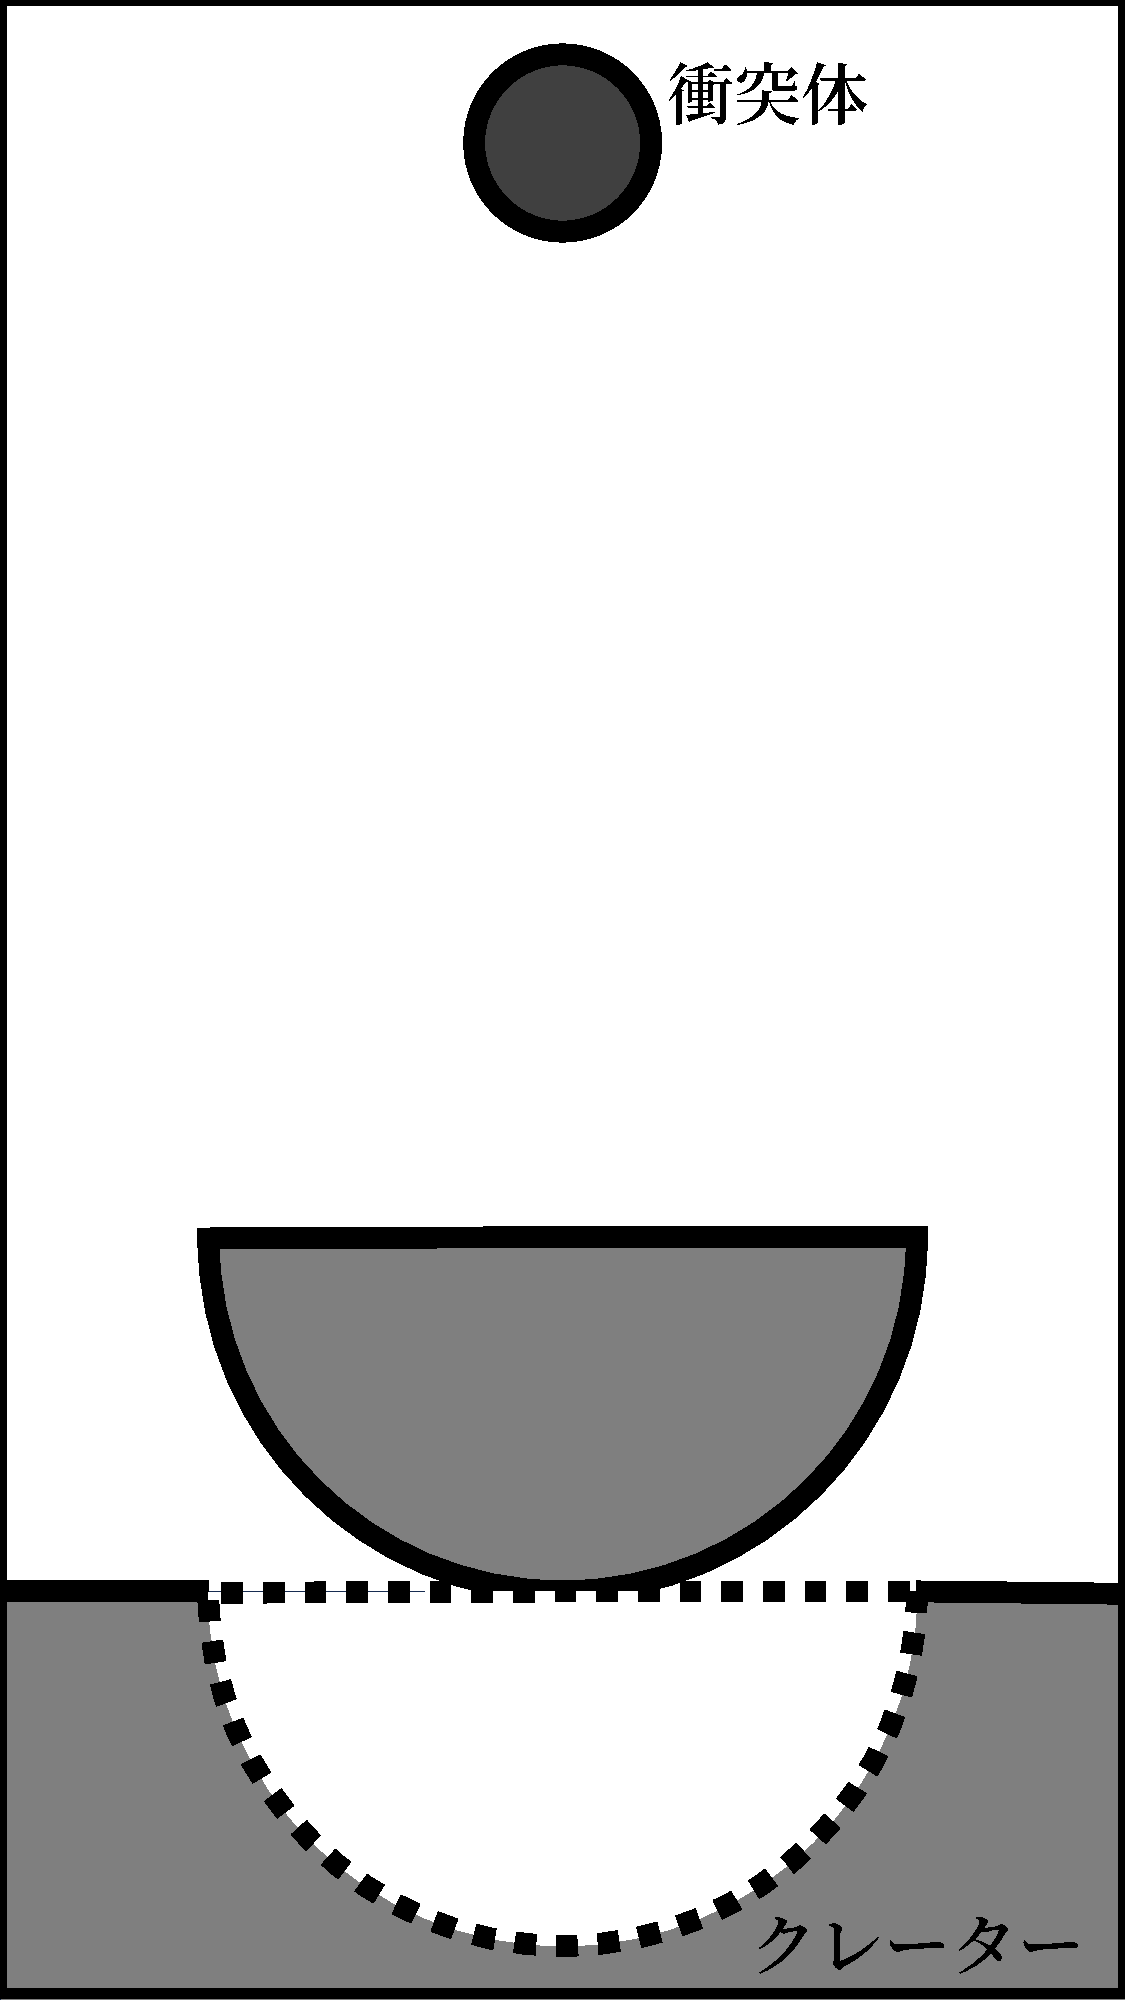
\includegraphics[width=80mm,clip]{./figure/explanation_figure.pdf}
    \vspace{-6mm}
    \caption{問題:参考図}
\end{wrapfigure}

今回のクレーターが半球であると近似してクレーター直径$D$と衝突エネルギー$E$の関係を求めてみよう。

砂の密度を$\rho$、重力加速度を$g$とする。クレーターをつくるためのエネルギーを、砂地の中の直径$2r$の半球をその半径の分だけそのまま持ち上げるエネルギーで近似する。なぜならば、クレーターができるためには、半球を埋めていた物質がその半球の外に出ていかなければならないからである。そのエネルギーは、半球の質量と$g$と半球の半径$r$の積で表される。おもりの衝突エネルギーがすべてこのエネルギーに変換されたと仮定すると次の等式が成り立つ。
\begin{equation}
    E = クレーターを作るためのエネルギー
\end{equation}

以上のことからクレーターの直径$D$と衝突エネルギー$E$の関係式を求めよ。

※裏面に回答してください。

※不明な点があれば遠慮なく担当者に質問してください。

\section*{参考文献}

\begin{itemize}
    \item 松井孝典. 2011. 比較惑星学. 地球惑星科学 12. 東京: 岩波書店.
    \item 佐々木晶, 土山明, 笠羽康正と大竹真紀子. 2019. 太陽・惑星系と地球. 現代地球科学入門シリーズ 1. 東京: 共立出版.
\end{itemize}

\end{document}